\documentclass[11pt]{report}
\usepackage{amsmath,amsthm,amssymb,wasysym}
\usepackage{mathtools}
\usepackage{enumerate}
\usepackage{graphicx}
\usepackage{mathpazo}
\usepackage{lmodern}
\usepackage{parskip}
\usepackage{fancyhdr}
\usepackage{wrapfig}
\usepackage{tikz}
\usepackage{hyperref}
\usepackage{listings}
\lstdefinestyle{MyPythonStyle}
{
    language=Python,
    basicstyle=\footnotesize,
    numbers=left,
    stepnumber=1,
    showstringspaces=false,
    tabsize=1,
    breaklines=true,
    breakatwhitespace=false,
}
\lstdefinestyle{MyCStyle}
{
    language=[Sharp]C,
    basicstyle=\footnotesize,
    numbers=left,
    stepnumber=1,
    showstringspaces=false,
    tabsize=1,
    breaklines=true,
    breakatwhitespace=false,
}
\usepackage[linesnumbered,algoruled,boxed,lined]{algorithm2e}
\usetikzlibrary{positioning, shapes.geometric, arrows}
\tikzstyle{startstop} = [rectangle, rounded corners, text centered, draw=black, fill=red!30]
\tikzstyle{io} = [text centered]
\tikzstyle{decision} = [rectangle, text centered, draw=black]
\tikzstyle{process} = [trapezium, text centered, draw=black]
\tikzstyle{arrow} = [thick,->,>=stealth]
\newtheorem{theorem}{Theorem}
\newtheorem{defn}{Definition}
\newcommand{\Jostle}{\texttt{Jostle}}
\newcommand{\dbspace}{\mathcal{R}}
\newcommand{\featspace}{\mathcal{X}}
\renewcommand{\t}[1]{\texttt{#1}}
\lhead{Senior Thesis}
\rhead{Jacob Imola}
\cfoot{\thepage}
\pagestyle{fancy}
\title{Automatic, Fine-Grained Algorithmic Choice for Differential Privacy}
\date{\today}
\author{Jacob Imola\\ School of Computer Science, Carnegie Mellon University\and Jean Yang\\ School of Computer Science, Carnegie Mellon University}
\begin{document}
\maketitle
\chapter{Introduction}\label{ch:intro}
The rapid technological increase in data collection, speed, and storage has brought about revolutionary insights and ideas and will continue to do so. However, with huge amounts of private data comes the concern of preventing data from ending up in the wrong hands. In order to prevent data leakage, we must lay a strong privacy foundation and give data programmers tools for implementing privacy both efficiently and correctly.

Consider a healthcare database with records like patient weight, age, genetic information, and whether they are HIV positive. Granting access rights, or policies, to just patients and their doctors protects as much privacy as possible, and developing tools for verifying information flow policies is an interesting question in its own right that has been studied immensely. However, sometimes it's okay to release some statistics about the database so that a programmer can find risk factors for people who have HIV. Publicly releasing the entire database doesn't protect privacy at all, yet it would be a programmer's dream. In order to appease both data programmers and patients, a middle ground area must be chosen where a blurry snapshot of the database is released, comprehensive enough so that meaningful conclusions may be drawn yet blurry enough so that individuals are mostly protected. We call this the \emph{privacy-accuracy} tradeoff. We can always sacrifice one for the other before we disclose our database snapshot. However, after we disclose, it is impossible to take any privacy back, so we have to be absolutely sure that privacy guarantee will not fail under any attack. The most promising method for doing such a disclosure is Differential Privacy~\cite{Dwork:2006}.

Differential Privacy (DP) is considered to be the gold-standard of privacy and has been researched intensely since its conception in 2005. Its goal is to provide guarantees on what can be done with the information being released from a dataset while making minimal assumptions about an attacker's abilities. Previous attempts at privacy were susceptible to surprise exploits that occurred after a database was released. Notably, before DP, researchers were able to reidentify users in a Netflix dataset given an auxiliary dataset from IMDB and form a generalized attack against the state-of-the-art privacy algorithms of the time~\cite{Narayanan:2006}. The strong privacy guarantee of DP, on the other hand, has a rigorous mathematical foundation that makes it impervious to the post-processing attacks that compromised the Netflix dataset, and more recently, \href{https://hackernoon.com/how-to-rob-an-airbnb-252e7e7eda44}{AirBnB} and \href{https://gizmodo.com/this-is-almost-certainly-james-comey-s-twitter-account-1793843641}{Instagram}. Differential Privacy has stood the test of time as a sturdy way to protect privacy.

However, just building a suite of DP algorithms is not satisfactory. Differential Privacy necessarily adds randomness to programs, and randomness adds a new layer of complexity to programs. For example, adding noise to a variable that governs how many times a loop is performed could result in two highly different program executions and thus a very noisy answer. However, in many DP applications, noise can be added in a number of places, different queries could be done to accomplish the same goal, and so on. A very noisy answer could potentially be avoided if the proper algorithm is deployed. If one algorithm always dominated the others, this wouldn't be much of a problem, but as we will see, the best one depends on the database in a complex way. Picking the best algorithm for the job depends on extensive empirical evaluations, as theoretical bounds are often insufficient for complex algorithms~\cite{Hay:2016}. This leads the central problem addressed by this work:

\textbf{Problem:} How can we alleviate the burden of empirical algorithmic choice from the programmer? 

This problem is noted by the authors of DPComp~\cite{Hay:2016}, who comment that currently, ``the practitioner is lost and incapable of deploying the right algorithm''. DPComp allows the programmer to visualize the performances of different histogram querying algorithms on certain datasets. An example of one algorithm executed on one dataset is shown in Figure~\ref{fig:dpcomp}. We feel this is a step in the right direction, but their approach would be better if its ideas were applied to a programming language. The approach is to move the manual exploration of algorithms that a programmer might do with DPComp into the runtime of our programming language, which we call \Jostle{}, so named because it will ``jostle'' the various algorithms during runtime. This will give the following benefits:

\begin{figure}
\begin{center}
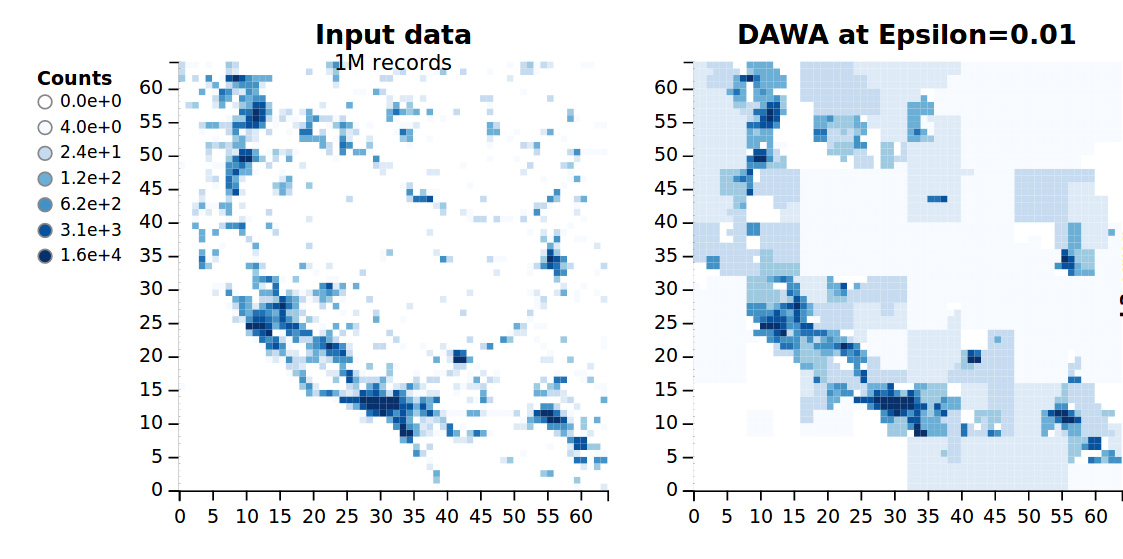
\includegraphics[scale=0.3]{DPComp}
\end{center}
\caption{A screenshot of a DPComp graph depicting the original dataset and the noise that a DP algorthm, DAWA~\cite{Li:2014}, adds at $\epsilon=0.01$. This would help a programmer decide whether to apply DAWA on his own dataset.}\label{fig:dpcomp}
\end{figure}
\begin{enumerate}
\item \textbf{Correctness} A \Jostle{} program enjoys the DP correctness guarantees that existing DP programming languages give. Correctness in the area of privacy is particularly important because privacy breaches are costly.
\label{itm:adv_correct}
\item \textbf{Generalization} The DPComp study of 2D histograms does not easily generalize to other DP algorithms. A programming language is far more general as arbitrary code can be analyzed. Concretely, DPComp can be implemented as a specific \Jostle{} program, and not the other way round.
\label{itm:adv_general}
\item \textbf{Differential Privacy Insight} DPComp is also a teaching tool because it advances one's knowledge of how algorithms perform on datasets. Every time a \Jostle{} program picks a algorithm, its trace extends a programmer's understanding of performance improves. This insight is particularly helpful to programmers new to DP who have no clues as to which algorithm to deploy.
\label{itm:adv_insight}
\end{enumerate}

Even though programming languages exist which confer benefit \ref{itm:adv_correct} and DPComp confers benefits \ref{itm:adv_general} and \ref{itm:adv_insight}, no works enjoy all three benefits at the same time. Having all three benefits is important because of programmer burden. Doing a DPComp-style analysis every time algorithmic choice needs to be explored requires doing data analysis on all algorithms and then implementing the insights by hand. Once algorithms are implemented, there is a small overhead writing \Jostle{} code to make the choice. The algorithmic insights come for free via the \Jostle{} trace.

\Jostle{} will represent algorithmic choice with the \t{MakeChoice} statement, illustrated in Figure~\ref{fig:1}.
\begin{figure}
\begin{lstlisting}[style=MyCStyle]
trainingSet = {US Census, ... #Public Databases}

uniformity = Feature(data){
    db = data.database
    xgrp = sqrt(db.x_range)
    ygrp = sqrt(db.y_range)
    return {{stddev(select sum(values) from db 
                    groupby x/xgrp, y/ygrp)}}
}
sparsity = Feature(data){
    db = data.database
    num_nonzero = {{select count(values) from db 
                    where values > 0}}
    domain_size = db.x_range * db.y_range
    return num_nonzero/domain_size
}

DAWA = Option(data){
    //DAWA Implementation
}
MWEM = Option(data){
    //MWEM Implementation
}

scoreFunc = Utility(data, answers){
    //compare answers to data.queries run on non-private data.answers
}

noisyHistChoice = MkChoiceMaker among {DAWA, MWEM}
                    informed by {uniformity, sparsity}
                    trained on trainingSet 
                    wrt ScoreFunc
def answerHistQueries(data):
    answers = noisyHistChoice(data)
\end{lstlisting}

\caption{\Jostle{} code demonstrating the use of \t{ChoiceMaker} object, called \t{noisyHistChoice}. In this case, the options are the \t{DAWA} and \t{MWEM} 2D Histogram algorithms.}
\label{fig:1}
\end{figure}
A programmer will use a \t{ChoiceMaker} when they are unsure of which choice to make at a certain point in their code; in the example, they are choosing between the algorithms \t{DAWA} and \t{MWEM}. The constructor, \t{MkChoiceMaker}, takes in a set of \t{Options}, a set of training databases, and a set of functions from the database to $\mathbb{R}$ called metafeatures.

The above design is inspired by DPComp. Suppose we are a programmer deciding whether to run the \t{DAWA} algorithm on a public dataset shown in Figure~\ref{fig:dpcomp}. We may notice that the input is a rather sparse and non-uniform---most of the points are 0 (white) and the non-zero points are clustered into groups. Indeed, this dataset is the population distribution for the southwest United States. We decide that these two properties adversely affect the performance for \t{DAWA}, as it predicts many of the white points incorrectly to have a nonzero value. Similarly, \t{sparsity} might affect the performance of \t{MWEM}, but not \t{uniformity}. The set of all properties that may impact performance are the \emph{metafeatures}. They are database properties that we pay attention to when we estimate algorithm performance.

\t{MkChoiceMaker} will train a model from the set of metafeatures to predicted algorithm performance. The resulting \t{ChoiceMaker} can be called on a private database. When this happens, the metafeatures are evaluated on the database and the \t{Option} with the highest estimated performance is dispatched.

We will begin with a background section on DP and related work. Then, we will present a formal outline of how \Jostle{} runs. Thirdly, we will implement Decision Tree choice with \Jostle{} and provide empirical evidence for the claimed benefits (Page~\pageref{itm:adv_correct}) of \Jostle{}. Finally, we will discuss future directions for \Jostle{}.

\chapter{Background}\label{ch:background}
\section{Differential Privacy}
Differential Privacy makes the following promise to data subjects: ``You will not be affected, adversely or otherwise, by allowing your data to be used in any study or analysis, no matter what other studies, data sets, or information sources, are available''~\cite{Dwork:2006}. To make this more formal, we must analyze two databases, $D$ and $D'$, differing in only one row which represents a database before and after a user participates. We call such databases neighbors. Suppose we are running a algorithm $\mathcal{M}$ on the database. If an attacker is able to discern with confidence $\mathcal{M}(D)$ and $\mathcal{M}(D')$, then this poses a privacy threat. The strength of this confidence is quantified a real number $\epsilon$ such that small $\epsilon$ corresponds to low attacker confidence. This means that deterministic algorithms are already unacceptable if it's possible for $\mathcal{M}(D) \neq \mathcal{M}(D')$. We necessarily must output a probability distribution, and once we view $\mathcal{M})(D)$ as a distribution, we can finally pin down the definition:

\begin{defn}
$\mathcal{A}$ satisfies $\epsilon$-DP if for all $D$ and $D'$ such that $|D-D'|_1=1$ and for all $o$ in the range of $\mathcal{M}$, 
\[\Pr\left(\mathcal{M}(D) = o \right) \leq e^{\epsilon} \Pr\left(\mathcal{M}(D')=o\right)\]
\end{defn}

There is also a more general definition that gives a weaker privacy guarantee: 

\begin{defn}
$\mathcal{M}$ satisfies $(\epsilon, \delta)$-DP if for all $D$ and $D'$ such that $|D-D'|_1=1$ and for all $o$ in the range of $\mathcal{M}$, 
\[\Pr\left(\mathcal{A}(D) = o \right) \leq e^{\epsilon} \Pr\left(\mathcal{M}(D')=o \right) + \delta\]
\end{defn}

For much of this paper, we will focus on $\epsilon$-DP, but it is worth knowing the more general case so we can import the well-known privacy theorems in their full generality.

The definition doesn't address why the ``no matter what'' part of the promise is true, but we can view any post-release attack on $\mathcal{A}$ as a function $F$ that doesn't involve $D$. Then, the following theorem establishes the promise:

\begin{theorem}
(Post-Processing~\cite{Dwork:2006}) If $\mathcal{M}$ satisfies $(\epsilon, \delta)$-DP, and $F$ is any function that takes the output of $\mathcal{M}$ as input, then $F(\mathcal{M})$ satisfies $(\epsilon, \delta)$-DP.
\end{theorem}
This theorem is the reason why DP is such a useful guarantee. Data programmers can be sure that once they run their algorithm $\mathcal{M}$ and release its output, then the DP guarantee gets no weaker \emph{no matter what an adversary does with the data}. This prevents the headaches where a programmer realizes retroactively that the data he released can be combined in some way to reveal much more information than was intended, like in Netflix~\cite{Narayanan:2006}.

In addition, DP satisfies several other useful properties:

\begin{theorem} \label{thm:comp}
(Composition~\cite{Dwork:2006}) Given algorithm $M_1$ and $M_2$ satisfying $\epsilon_1$ and $\epsilon_2$ DP, respectively, along with a database $D$, the algorithm $M = (M_1(D), M_2(D))$ has $(\epsilon_1+\epsilon_2, \delta_1+\delta_2)$ DP.
\end{theorem}
Composition is like the union bound from probability; it's convenient to apply but often is a pessimistic bound, as we will see later. Because of composition, we often refer to $\epsilon$ as a privacy budget---if we string together many private computations, it's like we spend some of our budget on each one out of a total budget of $\epsilon$.

We can easily improve upon Composition in the special case of algorithms operating on disjoint parts of the database. If $D$ is split into disjoint parts before algorithms are applied to it, then out of all its possible neighbors, only one of the parts will be different. Thus, only the worst algorithm will affect the DP guarantee:
\begin{theorem}\label{thm:disj}
(Disjointness~\cite{Dwork:2006}) Given disjoint subsets $D_1, D_2$ of $D$ with two algorithms $M_1$ and $M_2$ providing $(\epsilon_1, \delta_1)$ and $(\epsilon_2, \delta_2)$-privacy, then $((M_1(D_1), M_2(D_2))$ satisfies $(\max\{\epsilon_1, \epsilon_2\}, \max\{\delta_1, \delta_2\})$-DP.
\end{theorem}

So, what's a simple example of a DP algorithm? Suppose each row of our database $D$ is 0 or 1, so $D \in \{0, 1\}^n$, and that we are trying to release the sum of the elements of $D$. If this sum is $S$, then all neighboring databases $D'$ have sum $S$ or $S+1$. We can add noise to $S$ so that it looks very similar in distribution to $S+1$. The distribution we are looking for is the Laplace distribution:
\begin{defn}
The $\text{Laplace}(\lambda)$ distribution has probability mass function $f(x) = \frac{1}{2\lambda}e^{-|x|/\lambda}$.
\end{defn}
This distribution fits perfectly with the definition of DP because of the exponentials. If $X,Y$ are i.i.d. from $\text{Laplace}\left(\frac{1}{\epsilon}\right)$, then it is straightforward to show that the distributions of $S+X$ and $S+1+X$ satisfy $(\epsilon, 0)$ DP. To generalize this statement, we will use the following definition:
\begin{defn}
(Sensitivity) A function $f$ is $\Delta$-sensitive if for all $x,y$ such that $|x-y|_1 = 1$, we have 
\[
|f(x) - f(y)| \leq \Delta
\]
This can equivalently be rephrased as 
\[
\max_{|x-y|_1=1}|f(x) - f(y)| = \Delta
\]
We will denote the sensitivity of $f$ by $\Delta(f)$.
\end{defn}
This gives us the following algorithm:

\begin{algorithm}\label{alg:1}
\SetAlgoLined
\SetKwInOut{Input}{Input}\SetKwInOut{Output}{Output}
\Input{$D$, a database; $f$, a function $\mathcal{D} \rightarrow \mathbb{R}^n$; and $\epsilon$}
\Output{An estimate for $f(D)$ satisfying $\epsilon$-DP.}
$X$, a vector of $n$ i.i.d. variables drawn from $\text{Laplace}\left(\frac{\Delta(f)}{\epsilon}\right)$\;
\Return{X+f(D)}
\caption{Laplace Mechanism}
\end{algorithm}

\begin{theorem}
The Laplace mechanism~\ref{alg:1} satisfies $(\epsilon, 0)$-DP~\cite{Dwork:2006}.
\end{theorem}
For the counting or histogram queries such as our example above, we have $\Delta = 1$ so we add $\text{Laplace}\left(\frac{1}{\epsilon}\right)$ noise to our function.

However, what if we wanted to compute the maximum value in a set? If we had $n$ elements, we certainly wouldn't want to apply Composition $n$ times, obtaining $n\epsilon$-DP, just to have $\t{Laplace}\left(\frac{1}{\epsilon}\right)$ noise added to our answer. A better way is to use ReportNoisyMax~\ref{alg:max}. Instead of paying $n\epsilon$, ReportNoisyMax allows us to pay $\epsilon$ for the exact same noise on our answer.
\begin{algorithm}\label{alg:max}
\SetAlgoLined
\SetKwInOut{Input}{Input}\SetKwInOut{Output}{Output}
\Input{$D \in \mathcal{D}$, $\mathcal{X}$, a domain; $f$, a function $\mathcal{X} \times \mathcal{D} \rightarrow \mathbb{R}$; and $\epsilon$}
\Output{$x \in \mathcal{X}$ that attains maximum value on $f(S)$, satisfying $\epsilon$-DP.}
$X$, a vector of $|\mathcal{X}|$ i.i.d. variables drawn from $\text{Laplace}\left(\frac{\Delta(f)}{\epsilon}\right)$\;
\Return{$\arg\max_{i=1}^{|\mathcal{X}|}\{ X+f(\mathcal{X})\}$}
\caption{ReportNoisyMax}
\end{algorithm}
However, ReportNoisyMax only works on monotone queries, meaning $f(x, D) < f(x, D')$ for all $x \in X'$. A version that works on queries in general is the exponential mechanism~\ref{alg:exp}.
\begin{algorithm}\label{alg:exp}
\SetAlgoLined
\SetKwInOut{Input}{Input}\SetKwInOut{Output}{Output}
\Input{$D\in \mathcal{D}$; $\mathcal{X}$, a domain; $f : \mathcal{X}\times \mathcal{D} \rightarrow \mathbb{R}$, a utility function, $\epsilon$}
\Output{$x \in \mathcal{X}$ where $f(x, D)$ is more likely to be high.}
Pick $x \in \mathcal{X}$ where $\Pr(x=k) \propto \exp\left(\frac{\epsilon f(k, D)}{2\Delta(f)}\right)$\;
\Return{$x$}
\caption{exponential mechanism}
\end{algorithm}
ReportNoisyMax doesn't have a factor of 2 in its Laplacian noise, and this means a lighter tail. Thus, for monotone queries, we use ReportNoisyMax.
\section{Related Work}
\subsection{Existing Programming Languages}
Existing programming languages for differential privacy leave algorithmic choice up to the programmer. Languages with DP runtimes give the programmer certain DP primitives to use and compose them together~\cite{McSherry:2010}~\cite{Proserpio:2014}~\cite{Johnson:2017}. For example, in PINQ~\cite{McSherry:2010}, the primitives are aggregations, database splitting, and the exponential mechanism. Aggregations use the Laplace mechanism, and database splitting uses disjointness. To string together many commands, PINQ gives the user the ability to define a PINQAgent which keeps track of budgets in a compositional way. For example, the \t{NoisyCount} function is implemented in Figure~\ref{fig:PINQNoisyCount}.

\begin{figure}
\begin{lstlisting}[style=myCStyle]
double NoisyCount(double epsilon){
    if(myagent.apply(epsilon)){
        return mysource.Count() + Laplace(1.0/epsilon);
    }else{
        throw new Exception("Access Denied")
    }
}
\end{lstlisting}
\caption{NoisyCount Implemented in PINQ.}
\label{fig:PINQNoisyCount}
\end{figure}

If we wanted to count the number of patients in a database who are over 40, we would use \t{NoisyCount}, and an error would be thrown if the budget were to run out.

In Fuzz~\cite{Reed:2010}, a type system is implemented to guarantee differential privacy and sensitivity. Each type is endowed with a metric, and judgments are given for richer programming constructs such as sums, products, recursive types, and lambda expressions. Once the type of the program is known, its metric is known and its sensitivity can be inferred from the input variables. Sensitivity allows us to add the proper amount of noise via the Laplace mechanism. To go from an $\epsilon$-sensitive function to an $\epsilon$-DP function, noise is added via a monad by applying the function $add\_noise : \mathbb{R} \multimap M\;\mathbb{R}$.

For instance, counting the number of people in a database older than 40 could be achieved by:
\[
\lambda db.add\_noise\;(size\;(filter\;over_{40}\;db)) : db \multimap M\;\mathbb{R}
\]

The final type determined by Fuzz contains the differential privacy guarantee of the program. As opposed to throwing errors, Fuzz's sacrifice is making suboptimal typing judgments when computing the sensitivity as well as an undecidable type system. After all, there's no such thing as free lunch.

While algorithmic choice could be manually implemented in PINQ or Fuzz, this programmer burden will be eliminated in \Jostle{}. We design \Jostle{} to resemble PINQ with a \t{MakeChoice} construct rather than Fuzz because more accurate algorithmic choices can be done during runtime rather than compile-time.

\subsection{Existing Methods for Algorithmic Choice}

Versions of algorithmic choice have been demonstrated in previous work. Algorithmic choice involves picking an algorithm from a set that maximizes a score function. The problem can be set up in the following way: Given some answer space $\mathcal{M}$, a answer set $M \subseteq \mathcal{M}$, a database $D$, and a score function $q: \mathcal{R} \times \mathcal{M} \rightarrow \mathbb{R}$, maximize $q$ over $\mathcal{M}$ privately.

For instance, if the programmer is training a private logistic regression as an answer, then $\mathcal{M}$ is the space of all linear functions and $q$ is, most commonly, a validation score on some unused part of the database. This problem is extra subtle as changing $D$ to $D'$ changes the answer set from $M$ to $M'$, as the answers are determined on the database, and also changes $D$ to $D'$ when evaluating $q(D, m)$. There is no complete answer to this problem; most commonly, an assumption must be made about $q$, usually relating to its sensitivity. We now explore proposed solutions to this problem.

In~\cite{Chaudhuri:2013}, a solution based on the exponential mechanism is proposed where $q$ is the utility function used in the exponential mechanism. When we do this, we necessarily limit ourselves to manually picking $\epsilon$ both for the algorithms we are picking and for the final application of the exponential mechanism. We call this approach privacy-first, since privacy must be fixed first.

Since the exponential mechanism requires a sensitivity bound, a bound on $q$ must be ascertained. As mentioned, in order to bound $|q(D, m) - q(D', m')|$ where $m \in M$ and $m' \in M'$, two inequalities are needed:
\begin{align*}
\forall m\in M,\forall |D-D'|=1:\;\|q(D, m) - q(D', m)\| &\leq \beta_1 \\
\forall D\in \mathcal{R},\forall m \in M,\forall m'\in M':\;\|q(D, m) -  q(D, m')\| &\leq \beta_2
\end{align*}

If these bounds are established, then it's relatively easy to show that the exponential mechanism can output an answer that is close to optimal (compare to the guarantee of the exponential mechanism [Ask Matt about a citation for this]):
\begin{theorem}\label{thm:dependent_exp}
(Utility guarantee~\cite{Chaudhuri:2013}) Let $M = m_1, m_2, \ldots, m_k$. Then, with probability at least $1-\delta$, $q(D, m_{i^*}) \geq \max_{1\leq i \leq k} q(D, m_i) - \frac{2\max\{\beta_1, \beta_2\}\log(k/\delta)}{\epsilon}$.
\end{theorem}

Going back to the logistic regression example, a programmer may be unsure of which linear separator to pick as logistic regression depends on a hyperparameter. Therefore, they may split $D$ into a training set $T$ and validation set $V$. Then, they pick a set of hyperparameters $C$, set $M = \{w_D^{(c)}: c \in C\}$ and set 
\[
q(w, V) = -\frac{1}{|V|}\sum_{(x, y) \in V} g(w, x, y)
\] 
The function $g$ could be any function with bounded sensitivity; for instance, they could make it the logistic loss function $\log\left(1+e^{-yw^Tx}\right)$ which has sensitivity 1, so $\beta_1 = \beta_2 = 1$.

A small improvement to Theorem~\ref{thm:dependent_exp} is shown in~\cite{Chaudhuri:2014}. Suppose there is a relatively small subset of answers $M' \subseteq M$ which perform much better than the rest of $M$, so $\min_{m \in M'} q(D, m') \geq \max_{m \in M} q(D, m) + \delta$. It's possible to approximately find such an $M'$ with a complicated method called the sparse vector technique. With a smaller subset of better-performing algorithms, the exponential mechanism can be applied and the bound in Theorem \ref{thm:dependent_exp} will degrade proportionally to $\log{|M'|}$ rather than $\log{|M|}$.

Another example of a privacy-first framework is DPComp \cite{Hay:2016} and its extension, Pythia \cite{Kotsogiannis:2017}. DPComp allows programmers to visualize performances of histogram algorithms on public datasets so they can evaluate themselves which algorithm to deploy on their own dataset. The hope is that the programmer will know enough about their own dataset to find a similar public dataset and obtain an accurate visualization. An example visualization is shown in Figure~\ref{fig:dpcomp}.

Pythia takes this one step further in a similar way to \Jostle{}. A programmer will take ``features'' of their database---for example, the number of points, the number of zeros, the range of each database column---and Pythia will train a model that tells which algorithm does the best. Because of their simplicity and high interpretability, Pythia trains decision trees using algorithm runs gathered from public datasets. An example decision tree is shown in Figure~\ref{fig:pythia}. The leaves of the decision tree are the best algorithm to deploy, and the branches are comparisions done on the provided features.

\begin{wrapfigure}{r}{0.5\textwidth}
\begin{center}
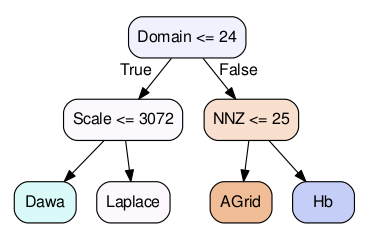
\includegraphics[scale=0.5]{PythiaDTree}
\end{center}
\caption{Example Decision Tree trained by Pythia with features in branches and algorithms in leaves.}\label{fig:pythia}
\end{wrapfigure}
On the other hand, the framework developed in~\cite{Ligett:2017} puts accuracy first. The programmer decides when accuracy is sufficiently high, and privacy usage is then minimized. Critical to the framework is the method of picking correlated Laplacian noise described in~\cite{Koufogiannis:2015}. In this version of the Laplace mechanism, a programmer selects a set of increasing $\epsilon$ values, $(\epsilon_1, \epsilon_2, \ldots, \epsilon_T)$, corresponding to the different budgets they want to try. Correlated Laplace variables $(v_1, v_2, \ldots, v_T)$ are then generated such that knowing a prefix $(v_1, v_2, \ldots, v_t)$ is $\epsilon_t$-differentially private and the noise present in $v_t$ is similar to the noise that a standard Laplace mechanism would add. The framework in~\cite{Ligett:2017} uses this algorithm to add noise to models $m_1, m_2, \ldots, m_T$ when the sensitivities of the models are known. For instance, if the task is linear regression, then the describing a way to iterate through the $v_i$'s until a suitably accurate algorithm is selected. Accuracy can be specified by the programmer as an arbitrary function that takes in a $v_i$. Of course, the release of the most-accurate algorithm has to be done in a differentially-private manner as well, and Ligett et. al use an adaptation of the AboveThreshold algorithm~\cite{Dwork:2006}. This results in an additional privacy and accuracy penalty over simply using the Laplace mechanism with a fixed $\epsilon$. Specifically, if $v_t$ is chosen, then the computation is $\epsilon_t+\epsilon_{Above}$-DP.

The first and third frameworks make assumptions about the algorithms, specifically the score function. Even though Pythia's algorithmic choice is similar to Jostle, Pythia is not a programming language. Pythia loses out on PL generality as mentioned in the Introduction. Indeed, we will see that Pythia and the other two frameworks can be implemented in \Jostle{} in Chapter \ref{ch:solution}.

Possibly more papers to talk about:~\cite{Winograd-Cort:2017},~\cite{Liu:2018},~\cite{Hsu:2014}.

\chapter{Solution Overview}\label{ch:solution}
\section{Formal Description}
Here, we describe in detail how \Jostle{} is implemented. Let the database space be $\mathcal{R}$, the metafeature space be $\mathcal{X}$, and the answer space be $\mathcal{M}$. $\mathcal{X}$ includes a private database as well as public information such as the number of columns in the database. Any argument passed to the algorithms is also included in $\mathcal{R}$, for example, 2D histogram queries to answer. \Jostle{} uses aggregations and database splits much like PINQ. More capabilities are possible as well as long as any time private data is touched, $\epsilon$ is specified. Additionally, \Jostle{} introduces the \t{Features}, \t{Option}, and \t{Score} types, and implements constructors with the following types:

\begin{center}
\begin{tabular}{|l|p{7cm}|}
\hline
Name & Type \\ \hline
\t{Features} & $\mathcal{R} \rightarrow \mathcal{X}$ \\ \hline
\t{MkFeatures} & $(\mathcal{R} \rightarrow x_i) \t{ list} \rightarrow \t{Features}$ \\ \hline
\t{Option} & $\mathcal{R} \rightarrow \mathcal{M}$ \\ \hline
\t{MkOption} & $\mathcal{R} \rightarrow \mathcal{M} \rightarrow \t{Option}$ \\ \hline
\t{Score} & $\mathcal{M}\times\mathcal{R} \rightarrow \mathbb{R}$ \\ \hline
\t{MkScore} & $\mathcal{M}\times\mathcal{R} \rightarrow \mathbb{R} \rightarrow \t{Score}$ \\ \hline
\t{Model} & $\mathcal{X} \rightarrow \mathbb{R}$ \\ \hline
\t{MkModel} & $(\mathcal{X} \times \mathbb{R}) \t{ list} \rightarrow \t{Model} $\\ \hline
\t{ChoiceMaker} & $\mathcal{R} \rightarrow \mathcal{M}$ \\ \hline
\t{MkChoiceMaker} & $\t{Option list} \times \t{Features}\times \mathcal{R} \t{ list} \times \t{TrainModel} \times \t{Score} \rightarrow \t{ChoiceMaker}$ \\ \hline
\end{tabular}
\end{center}
The functions of each type and the constructors are listed below:
\begin{itemize}
\item{\t{Features}} Created by \t{MkFeatures} which takes in a list of functions $f_1,f_2,\ldots,f_n$ where $f_i$ has type $\mathcal{R} \rightarrow x_i$. These are the feature-generating functions. The feature space is then $\mathcal{X} = \prod_{i=1}^n x_i$. \t{MkFeatures} will return a function that applies all $f_i$'s to a database and return the product.
\item{\t{Option}} Created by \t{MkOption} which takes in the implementation of the algorithm that the \t{Option} represents.
\item{\t{Score}} Created by \t{MkScore} which takes in the score function. The score function tells us, given an answer and possibly using the database, how well the answer did. Usually, the score will be model performance on a validation set.
\item{\t{Model}} Created by \t{MkModel}. This is the model which will learn a function from the features to the expected algorithm performance. A programmer could greatly change the performance of \Jostle{} by specifying different models, and different algorithmic insights could be revealed.
\item{\t{MkChoiceMaker}} Creates a \t{ChoiceMaker}. This constructor is the most complicated, and its implementation is shown in Figure \ref{fig:choicemaker}. First, models for all the inputted \t{Options} are trained. Then, a function returning the highest \t{Option} for an inputted database is returned. This function is the \t{ChoiceMaker}.
\end{itemize}

\begin{figure}
\begin{lstlisting}[style=MyPythonStyle]
def MkChoiceMaker(ops, feats, train_dbs, mkmodel, score):
    models = []
    for op in ops:
        xypairs = [(feats(db), score(db, op(db))) for db in train_dbs]
        models.append(mkmodel(xypairs))

    def GetAlg(db):
        feat = feats(db)
        perfs = [m(feat) for m in models]
        i = idxmax(perfs)
        return ops[i]
    return GetAlg
\end{lstlisting}
\caption{The implementation of \t{MkChoiceMaker}. }\label{fig:choicemaker}
\end{figure}
\section{Generality}
\subsection{Generality over PINQ}
\subsection{Generality over Ligett}
\subsection{Generality over DTree Algorithms}
\chapter{Experiments and Implementation}\label{ch:experiments}
\section{Decision Trees}

Decision Trees are a powerful tool for data mining due to their high human interpretability, non-parametric design, low computational cost, ability to discover non-linear relationships among attributes, resilience to missing values, ability to handle both discrete and continuous data, and ability to handle non-binary labels~\cite{Fletcher:2016}. Let our database again be $D$, and suppose it has $k$ columns or attributes, the $i$th of which can take values in $\mathcal{A}_i$. Let $\mathcal{C}$ be the output attribute, or class, which we are trying to predict. We assume for simplicity that $\mathcal{A}_i$ and $\mathcal{C}$ are discrete sets. A decision tree classifies points by branching on attribute $\mathcal{A}_i$, forming $|\mathcal{A}_i|$ subtrees. Once certain criteria are met, no more branching occurs, and instead a leaf node predicts the class. An example Decision Tree is given in Figure~\ref{fig:dt}.

\begin{figure}
\begin{center}
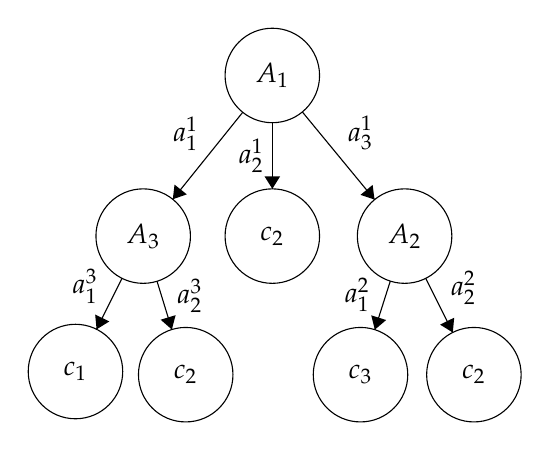
\begin{tikzpicture}[scale=0.2]
\tikzstyle{every node}+=[inner sep=0pt]
\draw [black] (18.1,-4.4) circle (3);
\draw (18.1,-4.4) node {$A_1$};
\draw [black] (9.9,-14.6) circle (3);
\draw (9.9,-14.6) node {$A_3$};
\draw [black] (5.6,-23.2) circle (3);
\draw (5.6,-23.2) node {$c_1$};
\draw [black] (12.6,-23.4) circle (3);
\draw (12.6,-23.4) node {$c_2$};
\draw [black] (18.1,-14.6) circle (3);
\draw (18.1,-14.6) node {$c_2$};
\draw [black] (26.5,-14.6) circle (3);
\draw (26.5,-14.6) node {$A_2$};
\draw [black] (23.7,-23.4) circle (3);
\draw (23.7,-23.4) node {$c_3$};
\draw [black] (30.9,-23.4) circle (3);
\draw (30.9,-23.4) node {$c_2$};
\draw [black] (16.22,-6.74) -- (11.78,-12.26);
\fill [black] (11.78,-12.26) -- (12.67,-11.95) -- (11.89,-11.33);
\draw (13.44,-8.08) node [left] {$a_1^1$};
\draw [black] (18.1,-7.4) -- (18.1,-11.6);
\fill [black] (18.1,-11.6) -- (18.6,-10.8) -- (17.6,-10.8);
\draw (17.6,-9.5) node [left] {$a_2^1$};
\draw [black] (20.01,-6.72) -- (24.59,-12.28);
\fill [black] (24.59,-12.28) -- (24.47,-11.35) -- (23.7,-11.98);
\draw (22.86,-8.07) node [right] {$a_3^1$};
\draw [black] (8.56,-17.28) -- (6.94,-20.52);
\fill [black] (6.94,-20.52) -- (7.75,-20.02) -- (6.85,-19.58);
\draw (7.05,-17.79) node [left] {$a_1^3$};
\draw [black] (10.78,-17.47) -- (11.72,-20.53);
\fill [black] (11.72,-20.53) -- (11.96,-19.62) -- (11.01,-19.91);
\draw (12.02,-18.37) node [right] {$a_2^3$};
\draw [black] (25.59,-17.46) -- (24.61,-20.54);
\fill [black] (24.61,-20.54) -- (25.33,-19.93) -- (24.38,-19.63);
\draw (24.33,-18.34) node [left] {$a_1^2$};
\draw [black] (27.84,-17.28) -- (29.56,-20.72);
\fill [black] (29.56,-20.72) -- (29.65,-19.78) -- (28.75,-20.22);
\draw (29.4,-17.89) node [right] {$a_2^2$};
\end{tikzpicture}
\caption{Example Decision Tree.}\label{fig:dt}
\end{center}
\end{figure}

The most widely-used algorithm for training decision trees is the C4.5 algorithm. C4.5 grows trees top-down, and it creates a branch up to a certain depth specified by the user. For each branch, it selects the attribute that produces the lowest conditional entropy and splits the dataset on it. Conditional Entropy is defined as:
\begin{defn}
(Entropy) The Entropy of a discrete random variable $X$ which attains $k$ values with probabilities $p_1, p_2, \ldots, p_k$ is
\[
H(X) = -\sum_{i=1}^k p_i \log(p_i)
\]
The conditional entropy of $X$ given a discrete random variable $Y$ which attains values $a_1, \ldots, a_\ell$ is
\[
H(X\mid Y) = \sum_{i=1}^\ell \Pr[Y=i] H(X\mid Y=i)
\]
\end{defn}
Conditional entropy, being a measure for information, is minimized so as to prioritize those attributes which produce large information gain. For leaf nodes, the class that has the largest representation in the remaining dataset is selected. The C4.5 algorithm appears in algorithm~\ref{alg:c45}.
We denote by $D^{(i)}_{x}$ to be the subset of $D$ which attains value $j$ on attribute $i$ and $D^{(i)}_{x,y}$ to be the subset of $D^{(i)}_{x}$ which also has class $y$. Let's let $\tau^{(i)}_{x,y}$ be the size of $D^{(i)}_{x,y}$. In the code, we represent this as \t{D[i=x]} and \t{D[class=y]}, respectively. Defining conditional entropy in our new notation, we get, for attribute with index $i$:
\begin{equation}\label{eq:cond_ent}
H_i(D) = 
\sum_{j\in \mathcal{A}_i} \frac{\tau^{(i)}_{j}}{\tau}\sum_{c \in \mathcal{C}} \frac{\tau^{(i)}_{j,c}}{\tau^{(i)}_{j}}\ln\left(\frac{\tau^{(i)}_{j}}{\tau^{(i)}_{j,c}}\right) \rightarrow \sum_{j\in \mathcal{A}_i}\sum_{c \in \mathcal{C}} {\tau^{(i)}_{j,c}}\ln\left(\frac{\tau^{(i)}_{j}}{\tau^{(i)}_{j,c}}\right)
\end{equation}
We omit a $\frac{1}{|D|}$ factor on the right side as we often simply compare computations on a fixed $D$. Two other estimates for the quality of a split which are generally less good in the non-private setting are Gini and Max:
\begin{align}
G_i(D) &= \sum_{j \in A_i} \tau^{(i)}_j\left(1-\sum_{c \in C}\left(\frac{\tau^{(i)}_{j,c}}{\tau^{(i)}_{j}}\right)^2\right)\label{eq:gini} \\
M_i(D) &= \sum_{j \in A_i} \max_c(\tau^{(i)}_{j,c})
\label{eq:max}
\end{align}
\begin{figure}

\lstinputlisting[style=MyPythonStyle, firstline=1, lastline=10]{./DTree.py}
\caption{C4.5 algorithm.}\label{alg:c45}
\end{figure}

When converting this algorithm to the differentially-private version, the user is left with several questions as noted in~\cite{Fletcher:2016}:
\begin{itemize}
\item How large of a budget has been alotted or should be alotted? There isn't a clear way to decide the budget, as the performance of the algorithm may vary wildly with the budget.
\item How many times should the data be queried? How would pick $d$ in C4.5? Should one alter line (1) to something different?
\item Might the sensitivity of some of the queries prevent an accurate choice? Specifically, even though it is widely agreed that the entropy function performs best in the non-private setting, could a lower-quality function be substituted because its computation is more accurate?
\item How does the size of $D$ impact performance? Is there enough data to provide accurate results in the private setting?
\end{itemize}
As we will see, the answers to these questions are data-dependent and the there is never one answer that always dominates.

\subsection{Private Decision Trees}
We assume, as does most of the literature, that the $\mathcal{A}_i$ and $\mathcal{C}$ are public and $D$ is private. Also, denote our total privacy budget to be $\beta$.
For recursive decision tree algorithms set up like~\ref{alg:c45}, the recursive calls on the same depth of the tree all operate on disjoint subsets of $D$. Therefore, a conservative estimate of the privacy usage, using composition and disjointness, is
\begin{equation}\label{eq:priv_est}
\sum_{i=0}^d \max_{n \in \t{Nodes on lvl }i} \epsilon_{n}
\end{equation}
where $\epsilon_n$ is the privacy used by node $n$. We will go into details on how to pick $\epsilon_n$ later.

The most naive way to create a DP version of C4.5 is to take all the histogram queries in algorithm~\ref{alg:c45} and change them to \t{NoisyCount}. This amounts to computing the dataset size, the most common class of a leaf, and the conditional entropy~\ref{eq:cond_ent} of a branch. Due to the disjointness of the $D^{(i)}_{j,c}$ with each other and the $D^{(i)}_j$ with each other with a fixed $i$, we can do a noisy count on each $|D^{(i)}_j|$ and $|D^{(i)}_{j,c}|$ with $\frac{\epsilon'}{2}$ budget (sensitivity 1), and compute the conditional entropy spending just $\epsilon'$ budget. Unfortunately, doing this over all attributes is not disjoint, so we have to split our $\epsilon_n$ budget over up to $k$ attributes and use composition. This adds a lot of noise to our computations, namely each NoisyCount gets $\frac{\beta}{dk}$ budget. This method is presented in~\cite{Blum:2005} as a proof of concept rather than a high-performing algorithm.

To fix this accuracy problem, Friedman and Schuster~\cite{Friedman:2010} use entropy as a utility function on a call to the exponential mechanism. Specifically, they operate over the domain $\{1,2,\ldots, k\}$, the indices of the attributes, and utility function $u(D, i) = -H_i(D)$, where the entropy is negated because we want to find the attribute with greatest entropy reduction. They also try functions other than entropy as a quality estimator because entropy has a rather high sensitivity, shown in Theorem~\ref{thm:ent_sens}.

\begin{theorem}\label{thm:ent_sens}
The entropy function on disjoint histogram counts $a_1,a_2,\ldots, a_n$ produced from a database $D$ has sensitivity bounded by $\frac{1}{|D|}\left(\frac{1}{\ln(2)} + \log(|D|) \right)$.
\end{theorem}
\begin{proof}
Let $A = \sum_{i=1}^n a_i$. Then, the entropy is 
\[
\sum_{i=1}^n \frac{a_i}{A}\log\left(\frac{A}{a_i}\right) = \frac{1}{A}\sum_{i=1}^n a_i\log A - \frac{1}{A} \sum_{i=1}^n a_i\log(a_i) = \log(A) - \frac{1}{A}\sum_{i=1}^n a_i\log(a_i)
\]
Suppose bucket $a_j$ is reduced by 1, and the entropy change is
\begin{align*}
&\log(A) - \log(A-1) - \frac{1}{A} a_j\log(a_j) + \frac{1}{A-1} (a_j-1)\log(a_j-1) \\
&\leq \frac{1}{\ln(2)(A-1)} -\frac{1}{A}(a_j-1)\log(a_j-1) + \frac{1}{A-1}(a_j-1)\log(a_j-1) \\
&= \frac{1}{\ln(2)(A-1)}+\frac{1}{A(A-1)}(a_j-1)\log(a_j-1) \leq \frac{1}{\ln(2)(A-1)} + \frac{1}{A}\log(A)
\end{align*}
\end{proof}
Another big change is the stopping criteria (Line 2 in Figure~\ref{alg:c45}). As noted in~\cite{Fletcher:2016}, the stopping criteria could be different in differential privacy versus the regular setting because $\text{Laplace}\left(\frac{1}{\epsilon}\right)$ creates much higher error in smaller leaves, and the depth of a tree affects the amount noise added. On a high level, this suggests that shorter, sparser trees will perform better in the DP setting, but the ultimate relationship remains unclear. In~\cite{Friedman:2010}, an additional stopping parameter depending on the NoisySize of $D$ and some other public parameters are used in addition to the stopping parameters in C4.5. Their goal is to ensure that a certain signal is larger than the noise of NoisyCount:
\[
\frac{|D|}{t|C|} < \frac{\sqrt{2}}{\epsilon}
\]
where $\frac{|D|}{t|C|}$ is a signal for how large the partitions that the children nodes will make. The sizes of $D$ for each node is used again when doing the standard C4.5Prune algorithm~\cite{Quinlan:1993} which doesn't use a validation set but estimates a confidence interval from the results of the training set. To do this, it needs an estimate on the sizes of $D[class=c]$ for each $C \in \mathcal{C}$ at each node, and knowing the size of $D$ helps Friedman and Schuster estimate this. Their algorithm is shown in Figure~\ref{alg:pc45}.
\begin{figure}
\lstinputlisting[language=Python, firstline=12, lastline=28]{./DTree.py}
\caption{Private C4.5 proposed by Friedman and Schuster~\cite{Friedman:2010}. } \label{alg:pc45}
\end{figure}
We've seen that Friedman and Schuster make three big design choices that are based on experimentation and heuristics:
\begin{itemize}
\item \textbf{Stopping Criteria} The \t{if} statement on Line 4 decides whether to continue branching or to stop, and in particular, the comparison of the signal to the noise is, in the words of the authors, ``arbitrary''. Also, the second pass done in \t{C4.5\_Prune} (Line 17) may clip a branch and is based on the noisy sizes collected in Line 3. 
\item \textbf{Non-Leaf Queries} For nodes that are not leaves, the exponential mechanism is used with different utility functions. The question of which utility function to use arises, as this is unclear given their different sensitivities.
\item \textbf{Number of Trees} It's well-known that a decision forest $\tau$ trees and a simple majority vote can often outperform a single decision tree. The number of trees to train in the DP setting could be much different than the answer in the non-private setting.
\end{itemize}
Another very important question is how much privacy budget to give to each of these components. If we give $0$ budget to the exponential mechanism, then we are essentially picking a random attribute. Random decision forests have been known to outperform decision trees in the non-private setting.
A summary of other works and their decisions on the above three criteria appear in the table below:
\begin{center}
\begin{tabular}{|p{2cm}|p{3cm}|l|p{3cm}|l|l|l|}
\hline
\; & Stopping Criteria in addition to $d = 0 || k=0$& $\epsilon_{stop}$ & Non-Leaf-Queries & $\epsilon_{NLQ}$ & $\epsilon_{LQ}$ & $\tau$ \\ \hline
Friedman \& Schuster~\cite{Friedman:2010} & $\frac{D}{t*|C|} < \frac{\sqrt{2}}{\epsilon}$; $d'$ user-defined; second pass with C4.5Prune & $\frac{\beta}{2d'}$ & Exp. Mech with entropy, Gini, max & $\frac{\beta}{2d'}$ & $\frac{\beta}{2d'}$ & 1 \\ \hline
Mohammed et al.~\cite{Mohammed:2015} & $d'$ user-defined & 0 & Exp. Mech with entropy & $\frac{\beta}{d'}$ & $\frac{\beta}{d'}$ & 1 \\ \hline
Jagannathan et al.~\cite{Jagannathan:2009} & $d'=$ min of $\frac{k}{2}$ and $\log_b(|D|)-1$ & 0 & Random & 0 & $\frac{\beta}{\tau}$ & 10 \\ \hline
Patil \& Singh~\cite{Singh:2014} & $\frac{D}{t*|C|} < \frac{\sqrt{2}}{\epsilon}$; $d'$ user-defined; second pass with C4.5Prune & $\frac{\beta}{2d'}$ & Exp. Mech with entropy & $\frac{\beta}{2d'\tau}$ & $\frac{\beta}{2d'\tau}$ & 10 \\ \hline
Fletcher \& Islam~\cite{Fletcher:2015} & $\log_b(|D|) < \frac{\sqrt{2}|C|}{\epsilon}$ & 0 & Random & 0 & $\frac{\beta}{\tau}$ & $m$ \\ \hline
\end{tabular}
\end{center}
Mohammed et al.~\cite{Mohammed:2015} propose not collecting the size (Line 3) and eliminating the size criterion on Line 4. This allows us to use the entire $\epsilon$ budget for the node on the exponential mechanism and on the NoisyCount (Lines 10 and 6, respectively). Jagannathan et al.~\cite{Jagannathan:2009} propose choosing a random attribute on Line 9, spending no budget, and setting $d = \min\{\frac{k}{2}, \log_b(|D|)-1\}$ where $b$ is the average branching factor of the attributes, $\frac{1}{k}\sum_{i=1}^k |\mathcal{A}_i|$. Patil and Singh~\cite{Singh:2014} do the same thing as Fletcher and Schuster but use multiple trees. Finally, Fletcher and Islam~\cite{Fletcher:2015} do random trees but without a predefined depth; instead, they estimate the support at each node by assuming that datapoints are cut uniformly at each branch, and they stop when the support is less than the noise, similar to Friedman and Schuster.

\subsection{Experiments}
In this section, we plot the performances of the five algorithms on different datasets to highlight the existence of data dependence. Graphs of the data for different datasets appear in Figure~\ref{fig:datadep}. The datasets are described below:
\begin{center}
\begin{tabular}{|p{3cm}|l|l|l|l|}
\hline
Name & No. Points & No. Attrs & Avg. Branch Size & Class size \\ \hline
HIV-1 protease cleavage & 1625 & 8 & 20 & 2 \\ \hline
Nursery & 12960 & 8 & 3.375 & 5 \\ \hline
Contraceptive & 1473 & 9 & 4.88 & 3 \\ \hline
\end{tabular}
\end{center}
The HIV dataset is a sparse dataset; there are far more possible attribute values than the number of data points actually in the dataset. As we go farther down the decision tree, after only a short while, the vast majority of nodes will have no training data at all---after just 3 branches, there are $20^3$ possible nodes which means almost $80\%$ of the nodes have to be empty, and most of the nodes have large support [insert a graph of this]. As is well known in decision trees, low-support nodes give noisier estimates of the classes, and it rarely pays to branch at these nodes. This explains the performances of the algorithms: A1, having the most sophisticated stopping criteria, performs the best because it knows which nodes have low support. A2, having almost no stopping criteria at all, performs the worst (and takes the longest to train, going to all $20^d$ leaves), and A5, with a stopping criterion almost as weak, took too long to train.

The Nursery dataset, on the other hand, is dense. The stopping criteria does not matter as much as all nodes have a healthy support (in fact, the dataset has points for every possible value of the attributes). Thus, A2, which doesn't waste any budget on the stopping criterion, performs best.

The Contraceptive dataset is a mix between the two other datasets. Here, one advantage of A3 is very pronounced: its excellent performances at small values of $\epsilon$. A3 gives the most budget to its leaf nodes, resulting in very accurate predictions at even small $\epsilon$ assuming the random trees are chosen in a fairly simple way. Because Contraceptive has no ``bogus'' attributes [insert graph of this], a randomly-chosen subset of the attributes is a fair set to work with, until the other, biased algorithms have enough budget to catch up.
\begin{figure}
\begin{center}
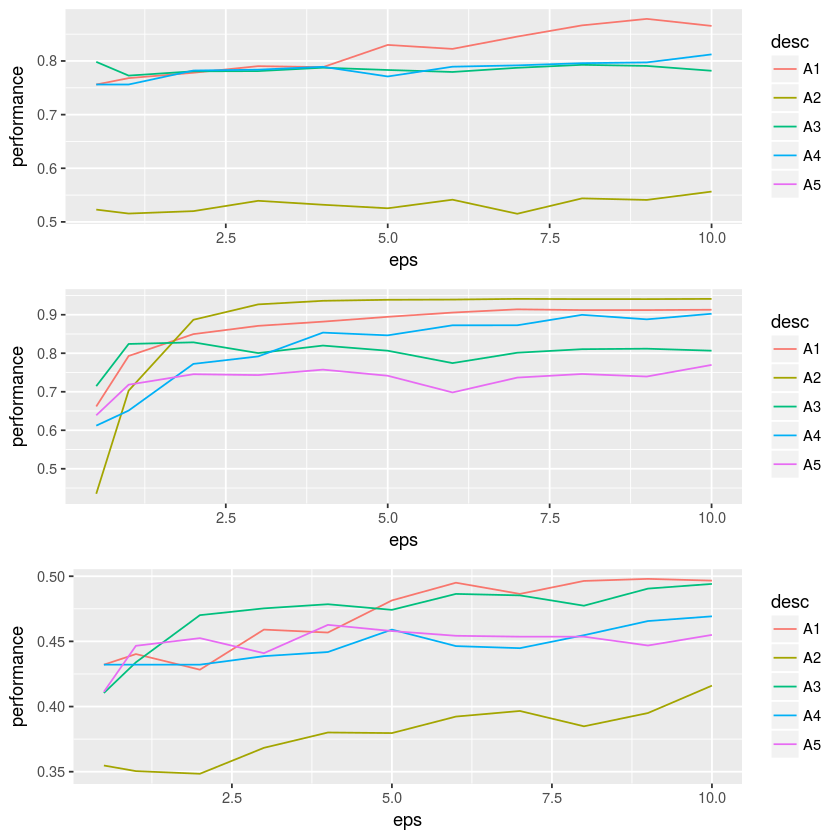
\includegraphics[scale=0.7]{Graph_Performances}
\end{center}
\caption{Performances of the five decision tree algorithms. The performance is measured from the prediction success rate on a validation set using a 30/70 validation to training split. Graph 1 does not have A5 because it takes such a long time to train, having a weak stopping criterion.}
\label{fig:datadep}
\end{figure}

In light of these experiments, we notice that stopping criteria, non-leaf-queries, and number of trees in the forest have a huge impact on the performance of the algorithm. What a programmer would really like to do is to shed light on these complicated relationships in an automated way. It would be easy for her to summarize all of the decision tree algorithms in a chart as in Figure~\ref{alg:dtree}. Each of the two places where she is uncertain is marked with a label, L1 or L2. The goal of \Jostle{} is to learn automatically properties of the database that may lend to a certain decision at L1 or L2.

Our goal is to decide which of the heuristics provided by all the decision trees may perform best, along with any other heuristic the programmer may provide us. 

\begin{figure}
\begin{center}
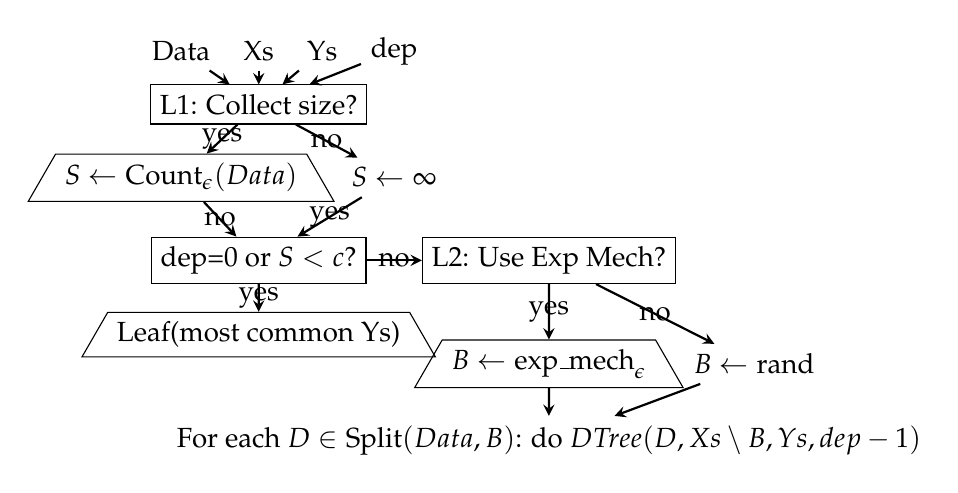
\begin{tikzpicture}[node distance=2cm]
\node (data_in) [io] {Data};
\node (xs_in) [io, right=0.5em of data_in] {Xs};
\node (ys_in) [io, right=0.5em of xs_in] {Ys};
\node (dep_in) [io, right=0.5em of ys_in] {dep};
\node (L1) [decision, below=0.5em of xs_in] {L1: Collect size?};
\draw [arrow] (data_in) -- (L1);
\draw [arrow] (xs_in) -- (L1);
\draw [arrow] (ys_in) -- (L1);
\draw [arrow] (dep_in) -- (L1);
\node (collect_yes) [process, below=3em of data_in] {$S \leftarrow \text{Count}_\epsilon(Data)$};
\node (collect_no) [io, below=3em of dep_in] {$S \leftarrow \infty$};
\draw [arrow] (L1) -- node {yes} (collect_yes);
\draw [arrow] (L1) -- node {no} (collect_no);
\node (stop) [decision, below=6em of xs_in] {dep=0 or $S < c$?};
\draw [arrow] (collect_no) -- node {yes} (stop);
\draw [arrow] (collect_yes) -- node {no} (stop);
\node (stop_yes) [process, below=1em of stop] {Leaf(most common Ys)};
\node (stop_no) [decision, right=2em of stop] {L2: Use Exp Mech?};
\draw [arrow] (stop) -- node {yes} (stop_yes);
\draw [arrow] (stop) -- node {no} (stop_no);
\node (exp_yes) [process, below=2em of stop_no] {$B \leftarrow \text{exp\_mech}_\epsilon$};
\node (exp_no) [io, right=0.5em of exp_yes] {$B \leftarrow \text{rand}$};
\draw [arrow] (stop_no) -- node {yes} (exp_yes);
\draw [arrow] (stop_no) -- node {no} (exp_no);
\node (wrap_up) [io, below=1em of exp_yes] {For each $D \in \text{Split}(Data, B)$: do $DTree(D, Xs\setminus B, Ys, dep-1)$};
\draw [arrow] (exp_yes) -- (wrap_up);
\draw [arrow] (exp_no) -- (wrap_up);
\end{tikzpicture}
\end{center}
\caption{Our decision tree algorithm with NoisyConditionals which learn the execution path from past histories. Depending on what the NoisyConditionals say, this algorithm is capable of expressing all the decision tree algorithms in~\cite{Fletcher:2016}.}\label{alg:dtree}
\end{figure}
\chapter{Future Work}\label{ch:future}
We hope to extend our work to causal inference. \cite{Devlin:2017} We believe our approach is more general than Ashwin's work. We hope to implement synthesis.

Synthesis example:
\begin{lstlisting}[style=MyPythonStyle]
class DAWA(Option):
    def answer(db, queries):
        #DAWA Implementation
    def predict(F):
        valuation = F.uniformity * (1-F.sparsity)
        return valuation
class MWEM(Option):
    def answer(db, queries):
        #MWEM Implementation
    def predict(F):
        valuation = 1-(F.sparsity)^2
        return valuation
\end{lstlisting}

However, our insights may not be perfect, and this is where \Jostle{} can help. When public datasets are fed into \t{MkChoiceMaker}, traces on the algorithm are produced which the programmer can analyze and update features.synthesis on the metafeatures and \t{predict} methods is done to try to improve prediction accuracy. Perhaps \Jostle{} realizes that a more accurate prediction for \t{MWEM} is $0.9-(\t{sparsity})^{1.5}$. Or, perhaps it thinks a better definition for \t{sparsity} is the number of points more than one standard deviation higher than the mean. Or, perhaps it decides a metafeature \t{xyz} is better for predicting the accuracy of \t{MWEM}.

Feature Optimization
\bibliographystyle{plain}
\bibliography{Thesis}
\end{document}